\documentclass[11pt]{article}

\usepackage{amsmath}
\usepackage{geometry}
\usepackage{epsfig}
\usepackage{epstopdf}
\usepackage{float}
\usepackage{pstricks}
\usepackage{pst-node}
\usepackage{pstcol}
\usepackage{pst-grad}
\usepackage{pst-plot}
\usepackage{color}
\usepackage{multicol}
\usepackage{multirow}
\usepackage{lscape}
\usepackage{harvard}

\setcounter{MaxMatrixCols}{10}
\setlength{\parskip}{0.5cm}

\begin{document}

\title{ECN726 - Term Paper\\ Disease and Development: The Effect of Life Expectancy on Economic Growth\\ Daron Acemoglu and Simon Johnson}
\author{Dilsat Dalkiran Ozel}
\date{December 2013}
\maketitle
\section*{Introduction}
It is obvious that better health conditions raises the life expectancy of the individuals. There is also a growing consensus, yet inconclusive, that higher life expectancy stimulates the economic growth. As people become healthier, their life expectancy increases and this expectancy makes them more productive. Hence, to what extent improved life expectancy affects the economic growth and per capita GDP is a valid and interesting question. Therefore, in their paper, Acemoglu and Johnson question whether there is a remarkable effect of life expectancy on economic growth between 1940 and 1980. 

Basically, the authors emphasize two main implications of higher life expectancy which may be named as population effect and productivity effect. According to this, increased life expectancy brings about two main implication which move in the opposite direction. On one side, higher life expectancy increases the total population in the economy and this has a negative effect on per capita income. On the other side, it increases the total productivity of workers which in the end causes more accumulated capital stock. As a result, it leads to higher per capita income. From this perspective, the final effect of higher life expectancy depends on which of the implications dominates the other.

The major difficulty about analysing the effect of life expectancy on GDP per capita is that there is not a one-way relationship between these two. One can simply argue that developed countries invest on health system more than the other countries. Hence, it puts an upward pressure on life expectancy. Acemoglu and Johnson overcome this reverse causality issue by introducing a mortality instrument which constitutes the hearth of the paper. Yet, they still can not reach a precise conclusion about the existence of positive effect of life expectancy on economic growth. 

Despite the growing consensus about the effectiveness of life expectancy on economic growth, this weak result is disturbing enough. Hence, I asked the most prominent question one can ask to this kind of paper: How about trying another instrument? The idea behind this extension can be explained as follows: life expectancy is not only affected by better health conditions but also by the armed conflicts in the country. No matter how good the health system is, feeling insecure, more precisely being in a war or any kinds of armed conflicts may have a remarkable impact on life expectancy of individuals. Hence, instead of mortality rates, I decide to use armed conflict data as an instrument which is going to be my extension for this paper and for my term project.
\section*{Model Specification and Data}
The economic model is based on a Solow growth model with human capital. Acemoglu and Johnson estimate a log-linear equation of income per capita which can be written as below:
\begin{equation}
y_{it}=\pi x_{it}+ \gamma_{i} + \mu_{t} + Z'_{it}\beta + \epsilon_{it}
\end{equation}
where y is log income per capita, x is log life expectancy at birth, $\gamma$ is fixed effect which is a function of the parameters: $A_{i}$, TFP; $h_{i}$, human capital; $N_{i}$,total population (and employment); and $K_{i}$ or $s_{i}$, which are capital stock and saving rate respectively. Lastly, $\mu_{t}$ is time varying factors common across all countries, $Z_{it}$ is vector of other control variables. Here, as expected, $\pi$ is the parameter of interest. 

The authors mainly use two kinds of estimators: OLS and 2SLS. They start their estimations with OLS just to display the high correlation between life expectancy and GDP data. Later, they develop a predicted mortality instrument for life expectancy as they expect a close relationship between the life expectancy and mortality rate. The predicted mortality instrument is formulated based on the data about the distribution of disease a country has and the effects of global interventions towards those particular diseases.

\begin{equation}
M^{l}_{it} = \sum\limits_{d \in D} [(1-I_{dt})M_{di40}+I_{dt}M_{dFt}]
\end{equation}
where, $M^{l}_{it}$ is predicted mortality, $I_{dt}$ is dummy for intervention for disease d at time t, $M_{di40}$ is pre-intervention mortality (pre 1940) and $M_{dFt}$ is mortality rate from disease d at the health frontier.

First of all, descriptive statistics of important variables are summarized in  Table 1. Acemoglu and Johnson data includes 75 countries from Western Europe, Oceania, the Americas and Asia between 1940 and 1980 (or 2000). Most of the data is collected from UN Demographic Yearbooks and League of Nations. The diseases they used in their estimation are malaria, influenza, tuberculosis, cholera, typhus, plague, whooping cough, scarlet fever, diphtheria, measles, pneumonia, typhoid, smallpox and cancer.
\begin{figure} [H]
\centering
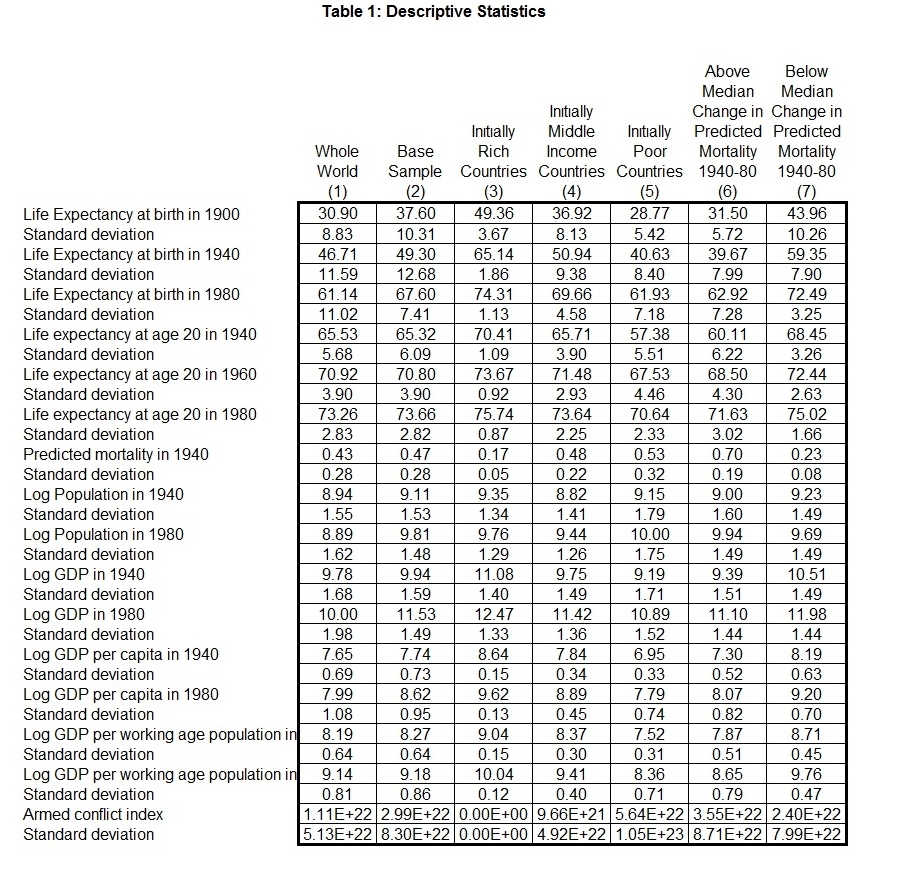
\includegraphics[width = \textwidth]{ds}
\label{table1}
\end{figure}
Different from their instrument, I am going use armed conflict index. I calculated this index by using the total days that a country is involved in an armed conflict and the conflict intensity. The data on armed conflict is prepared by a collaborated work by CSCW and Uppsala Conflict data program. The data includes the starting and ending dates of external and internal armed conflict for each country from 1946 to 2000. It also includes the intensity of each armed conflict which is categorized into 2 : one is low intensity meaning that the number of deaths are between 25 and 999. It is denoted with number 1. The other is high intensity which includes more than or equal to 1000 deaths and it is denoted with number 2. Briefly, number 2 means the country is in a war. Using the number of days and intensity data, I created a simple index for the armed conflict. 
\begin{equation}
index = \omega(days*1000)^{int_{1}} + (1-\omega)(days*25)^{int_{0}}
\end{equation}
where $\omega$ is a dummy variable indicating whether the country is in a war or not. If the country is in a war, $\omega=1$. $days$ is the total number of days passed in the armed conflict. I multiplied $days$ with $1000$ and $25$ because I assumed that if it is a war, at least 1000 people is going to die in a day. If it is an armed conflict at least 25 people is going to die in a day. Of course, the numbers come from the definitions of intensity mentioned above. Lastly, $int_{1}=2$ and $int_{0}=1$ which are the intensity of armed conflicts. If a country is involved in multiple armed conflicts in a year, I take the average of the indices for that year.

The main reason of this calculation is to emphasize the effect of armed conflict on individuals. If a country is in a war, no matter what the current health conditions are, individuals lower their life expectancy because they do not feel safe. Therefore, as the index for armed conflict gets bigger, life expectancy is going to go down. Hence, I am going to expect a lower productivity rate and a lower economic growth. One may call it as productivity effect. On the other hand, higher index will mean a destruction in human capital. Hence, population is going to decrease which may be translated into an increase in GDP per capita (say population effect). However, my initial assessment is productivity effect is going to dominate this population effect as I already magnify the effect of war with my calculation. In brief, using this new instrument, I am expecting to find the positive relationship between life expectancy and economic growth. 

\section*{Results}
\subsection*{Replication Analysis}
As the paper is really intense in terms of analysis, I have replicated 10 tables. I find it inconvenient to skip either of them as all the tables are related to each other. In general, I could replicate almost all the coefficients, number of observations, number of clusters correctly but I cannot claim the same thing for standard deviations and R squares. 

For my extensions, I only replicate table 8 and table 9 as they are the key tables of the paper.

Table 1 summarize the descriptive statistics of some key variables. You can find the same table with the same name in the original paper. The last two rows are means and standard deviations of my new instruments, armed conflict. As it is seen the numbers are quite high. In fact, the median is $1.3588E+14$ while the minimum number is $1000000$. I could squeeze the indices to a range between $1$ and $10$, as it is not going to give me a different result, I did not do it. 
\begin{figure} [H]
%\caption{Table 2: Life Expectancy, Population, Births, and Percentage of Population Under 20 - OLS Estimates}
\centering
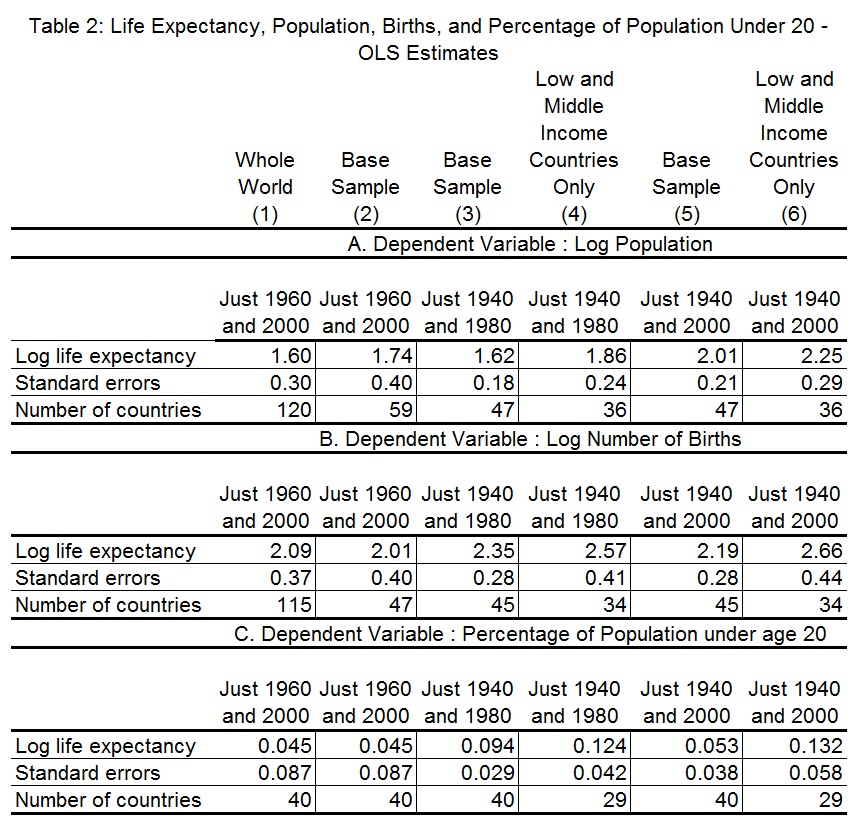
\includegraphics[width = \textwidth]{table2}
\label{table2}
\end{figure}
Table 2 shows the OLS estimations of log life expectancy on log population, log number of births and percentage of population under age 20. OLS regressions include full set of country and year fixed effects. We get rid of these fixed effect by taking the long differences. Standard errors are robust. I could replicate almost all the numbers but there are slight differences in column (6). Although the coefficients are the same, when the dependent variable is log population and log number of births, standard errors are slightly different. 
\begin{figure} [H]
%\caption{Table 3: Life Expectancy, GDP, GDP per capita and GDP per Working Age Population - OLS Estimates}
\centering
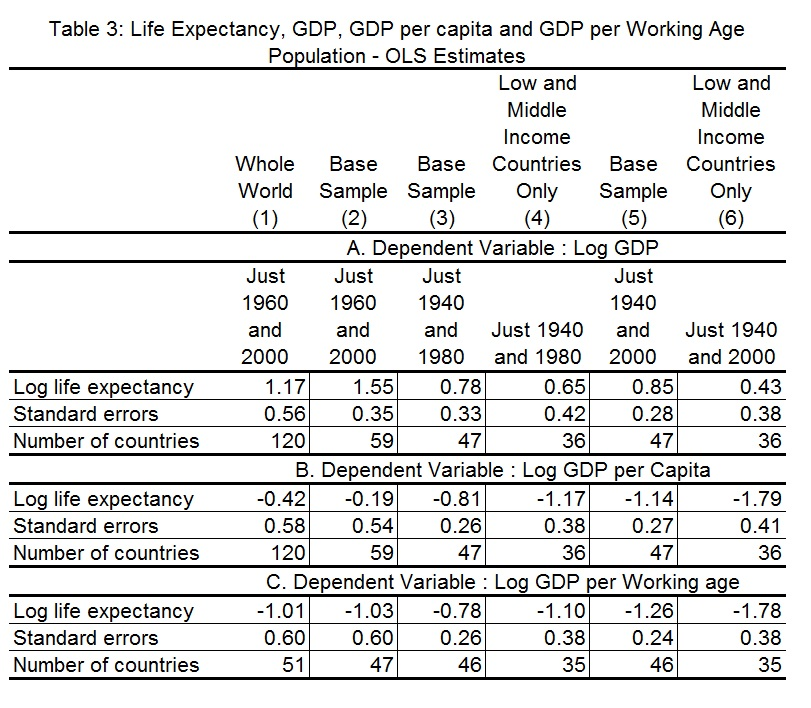
\includegraphics[width = \textwidth]{table3}
\label{table3}
\end{figure}
Table 3 is exactly replicated. In this table, we have shown the OLS estimations of log life expectancy on GDP, GDP per capita and GDP per Working Age Population. Standard errors are robust. As it is seen, there is a positive relationship between log GDP and log life expectancy. However, we cannot see the similar relationship when it comes to log GDP per capita and log GDP per working age population. According to authors claim, the main reason behind this inconsistency may be the reverse causality issue life expectancy and economic growth that is mentioned above. Hence, this becomes the main motivation for 2SLS estimations. 
\begin{figure} [h!]
%\caption{Table 4: Life Expectancy, GDP, GDP per capita and GDP per Working Age Population - OLS Estimates}
\centering
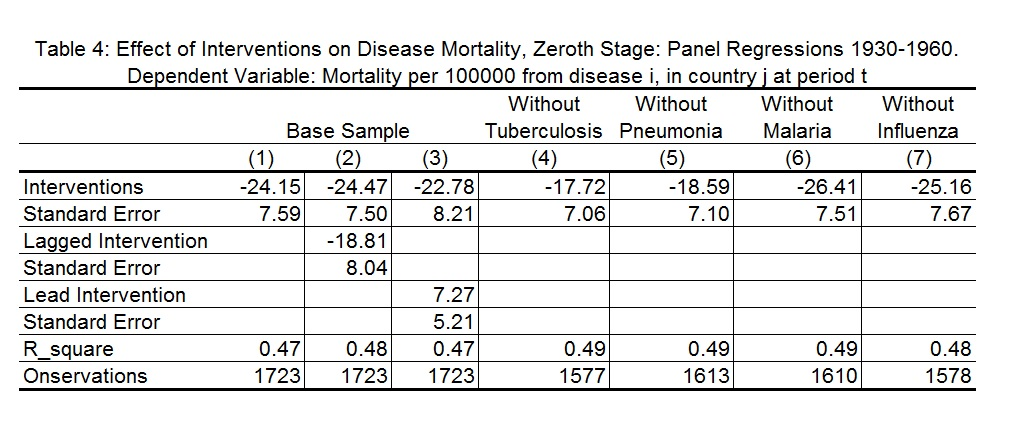
\includegraphics[width=\textwidth]{table4}
\label{table4}
\end{figure}
I could replicate almost all the coefficients, observation numbers and R squares in table 4 successfully. However, I could not replicate the papers results for standard errors. Although I adjusted robust standard errors by clusters, I could not find the same results. I followed Cameron and Trivedi book for the adjustment of standard errors. For that, I multiplied robust standard errors with $\frac{N-1}{N-K}\frac{C}{C-1}$ where N is the number of observations, C is clusters and K is the number of explanatory variables.
\begin{figure} [H]
\centering
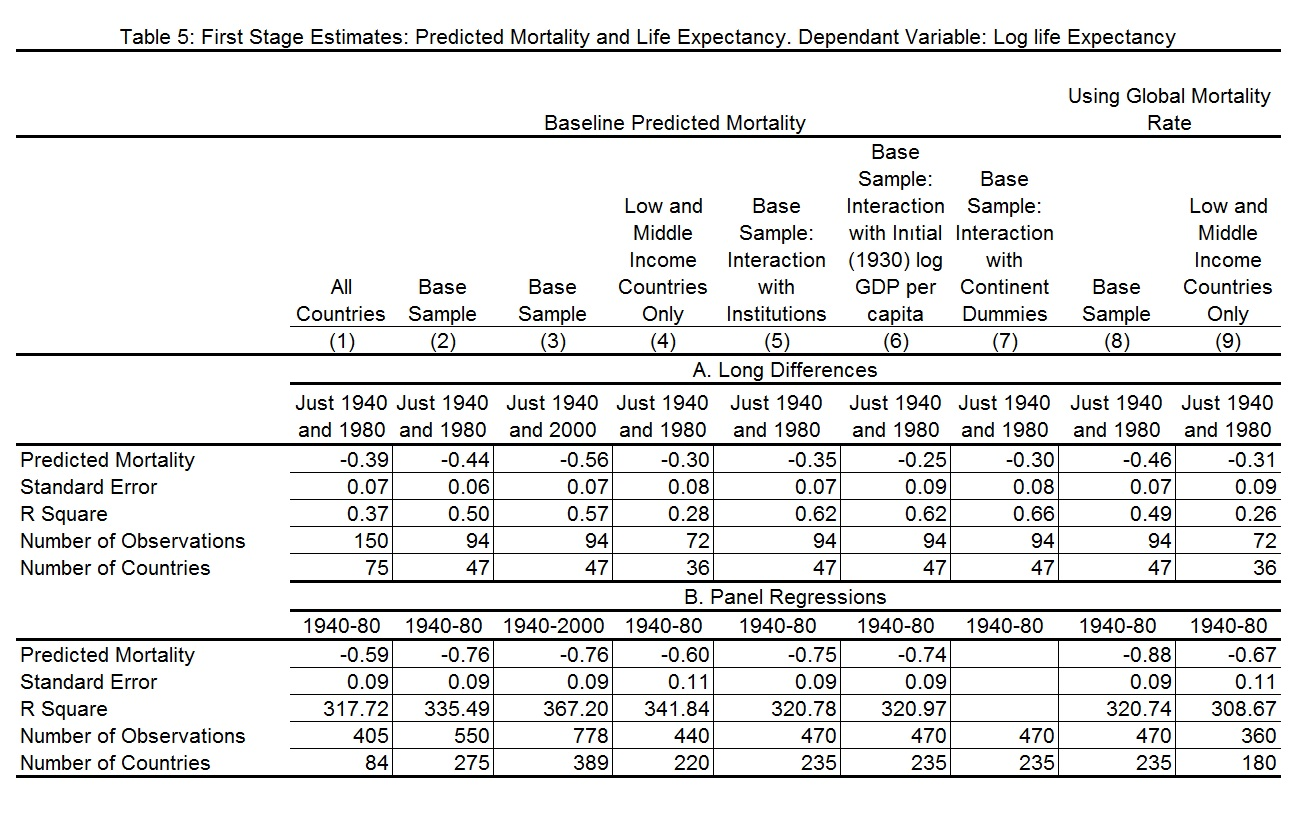
\includegraphics[width=\textwidth]{table5}
\label{table5}
\end{figure}
Table 5 shows the first stage estimates of predicted mortality and life expectancy. I replicated long differences estimations which is Panel A correctly. The only problem I encountered was that the R squares written in the paper are different from their Stata code which can be downloadable from Acemoglu's website. In the paper, the R squares are quite high but in their Stata code, we cannot say the same thing. Coming back to my estimations, I can state that comparing to what is written in the paper, my results are at least closer to Stata results. However, they are still different. I do not think that the authors made a mistake at this table but I think there must be some technical issue which I could not resolve due to time constraint.

Different from Panel A, the estimation result I have found for panel B is entirely different from the paper. By only examining the R square results I find, one can easily understand that I am making some technical mistake so I obtained this much of different result. 

The only table which I completely fail to replicate is Table 6. I cannot even post the table because I could not get any sensible result. Hence, I am not going to post it here but the code is available in my $m-file$. 
\begin{figure} [H]
\centering
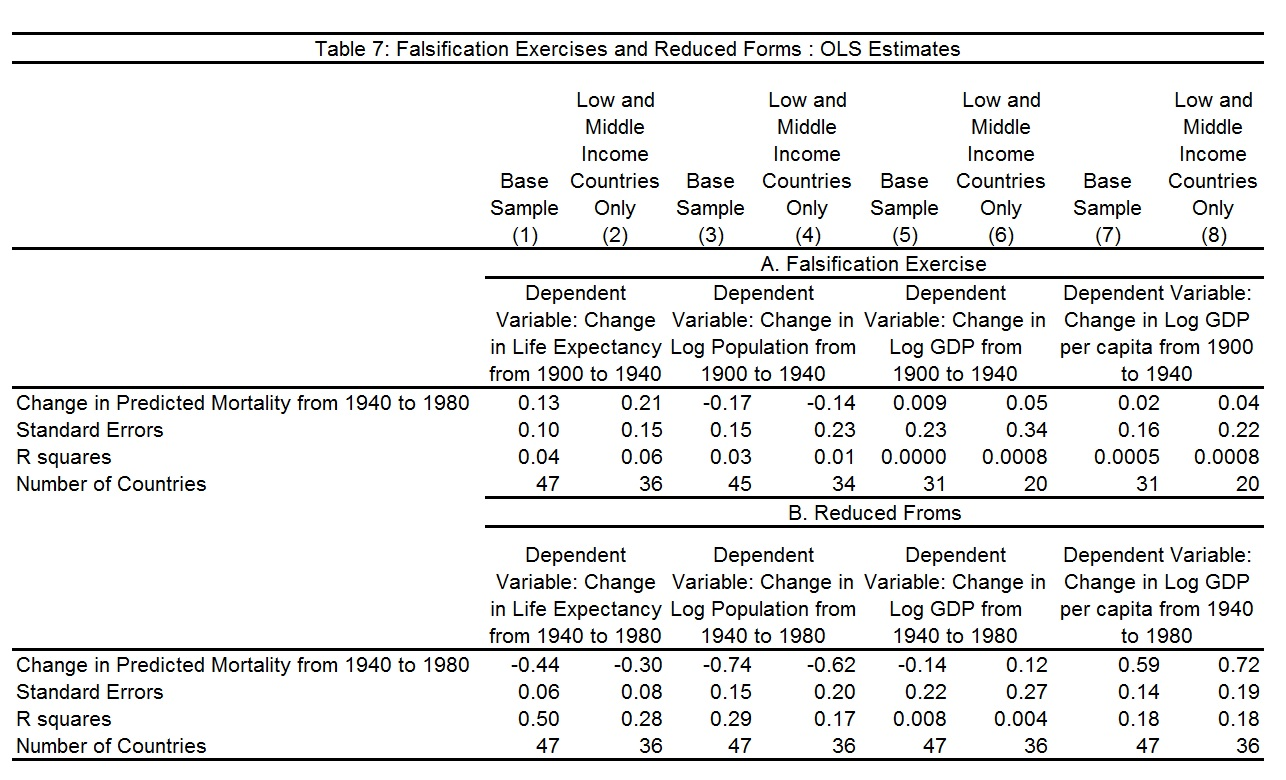
\includegraphics[width=\textwidth]{table7}
\label{table7}
\end{figure}
Table 7 displays some falsification exercises and reduced forms with OLS estimations. With some minor differences, I obtained almost exactly the same results. Here, the standard errors are also robust. On the other hand, there is again some inconsistencies with my findings and paper's standard errors. 
\\
Table 8 displays the effect of life expectancy on population variables. I could replicate most of the paper successfully but there are still inconsistencies between my standard errors and the paper's.
\begin{figure} [H]
\centering
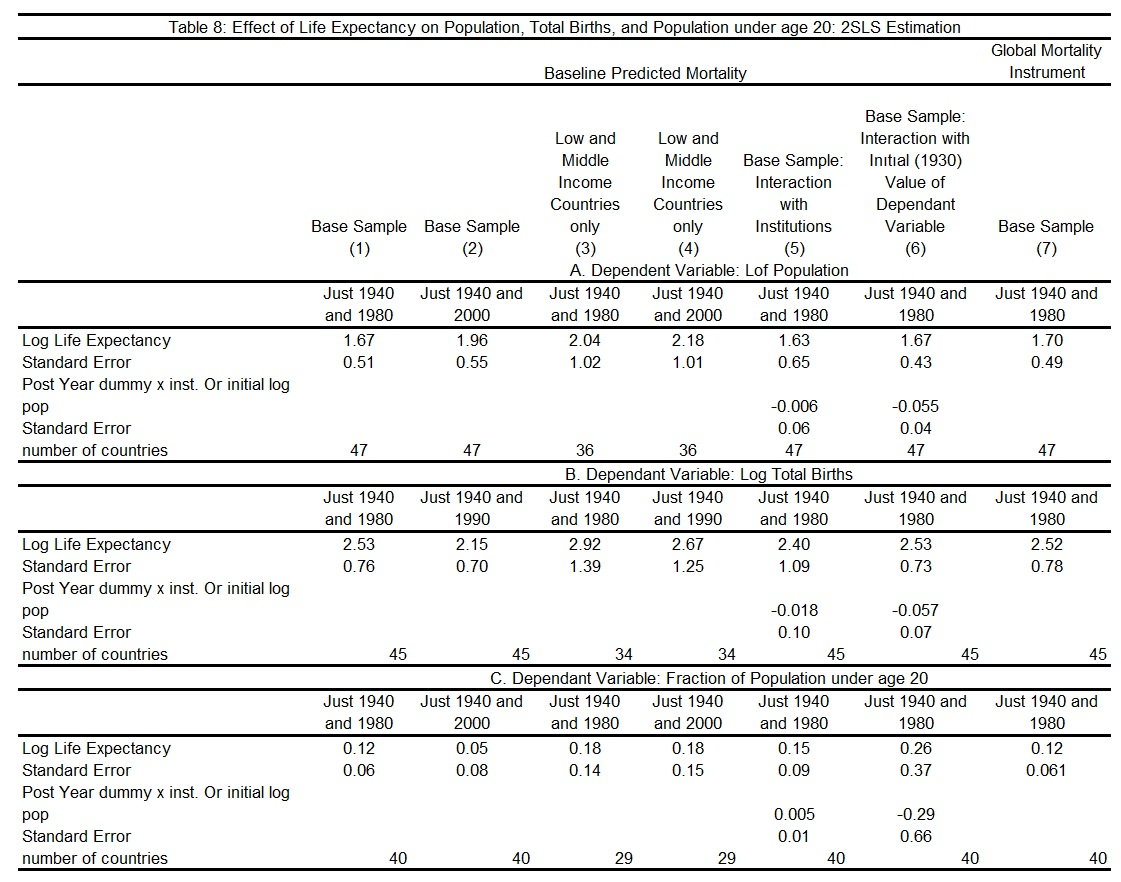
\includegraphics[width=\textwidth]{table8}
\label{table8}
\end{figure}
\begin{figure}
\centering
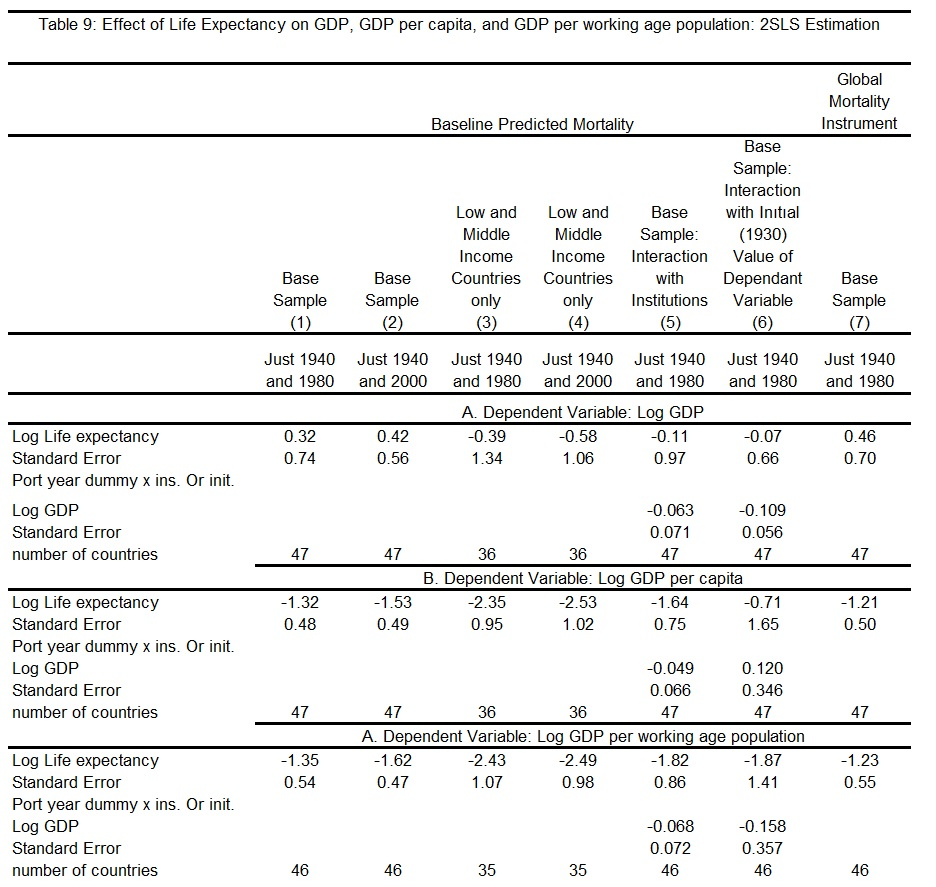
\includegraphics[width=\textwidth]{table9}
\label{table9}
\end{figure}
Table 9 displays the effect of life expectancy on GDP variables. As it is seen, even with the 2SLS estimations, there is a positive relationship between life expectancy and log GDP but negative relationship between life expectancy and log per capita GDP. Hence, population effect still seems more effective than the productivity effect. In this table, I could nor replicate standard errors correctly although I adjusted for clusters. Apparently, there is a chronic mistake I made in all of my Matlab code so I could sometimes reach the same standard errors and sometimes not.
\begin{figure} [H]
\centering
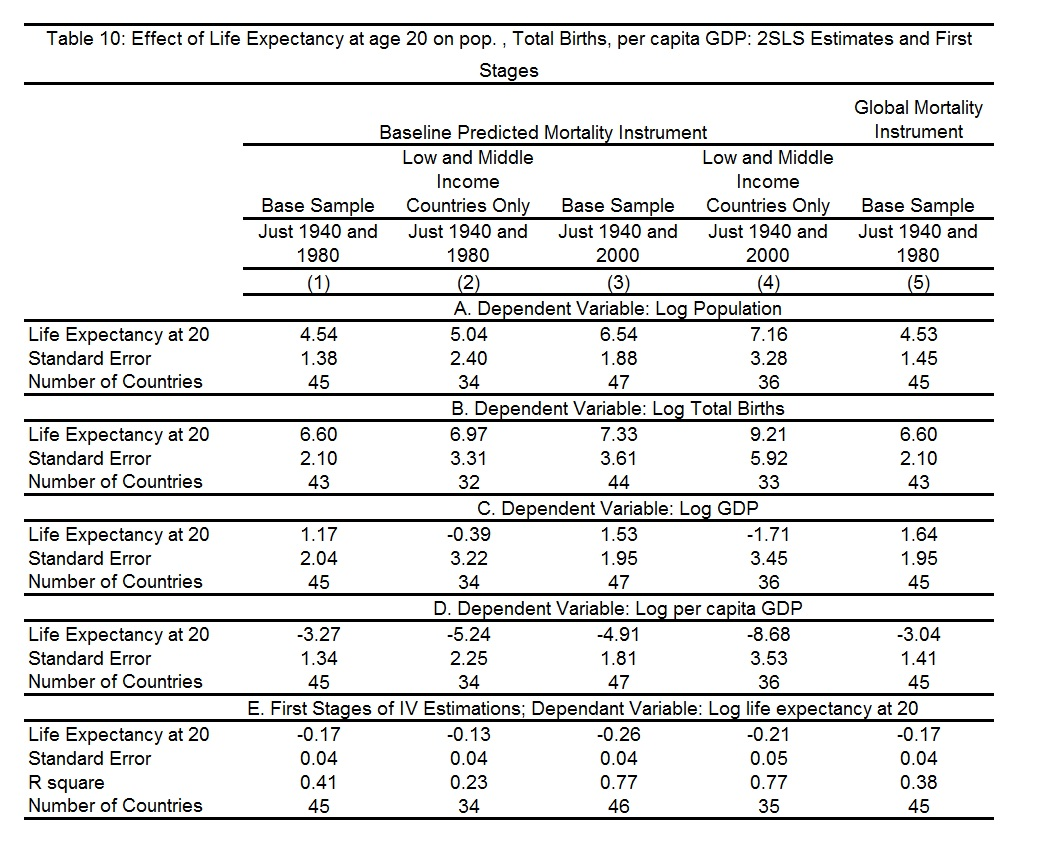
\includegraphics[width=\textwidth]{table10}
\label{table10}
\end{figure}
Table 10 is just the replication of the same analysis we did in table 8 and table 9. Different from them, this time we have an age constraint. However, this again does not change the ultimate conclusion. Moreover, we again have exaggerated R squares problem which I mentioned at table 5, as well.

As a result of these estimations, they could not reach that increase in life expectancy have a remarkable effect on economic growth as all its effect is dominated mostly by population growth.  It is correct that there is a close relationship between life expectancy and predicted mortality rate but as we have mentioned above, the mortality rate does not cause the growth effect of life expectancy to dominate the population effect. 

\subsection*{Extensions}
The main concern about the armed conflict index was whether it was a valid instrument or not. As the definition of income above already include some human capital and it is known that armed conflict may cause some destruction of human capital, it might create another reverse causality issue. One way to overcome this situation was to generate a non-linear transformation of the armed conflict data. Considering my definition of armed conflict index, I have get rid of this problem. I have proved that armed conflict index I created above is a valid instrument by conducting Sargan test. According to this test, I have shown that the instrument is valid. I get this conclusion by using Stata but unfortunately I could not replicate the same result by using Matlab. In any case, I am adding both of my results below and sent both $m-file$ and $do-files$. I completely believe Stata results and think that Matlab results are wrong due to some technical mistake, I proceed by relying on Stata result.
 \begin{figure} [H]
\centering
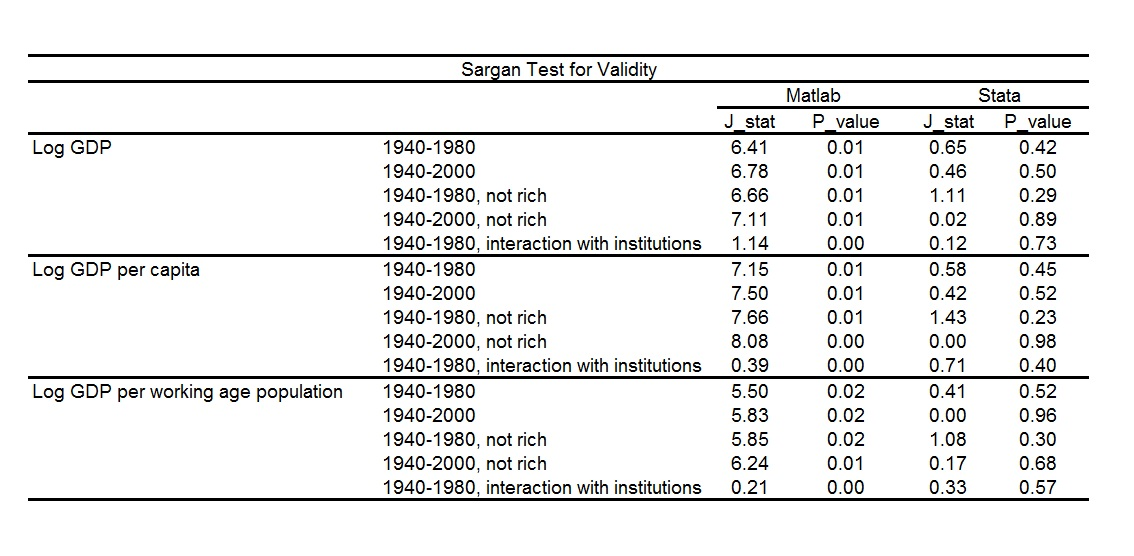
\includegraphics[width=\textwidth]{sargan}
\label{sargan}
\end{figure}

\begin{figure} [H]
\centering
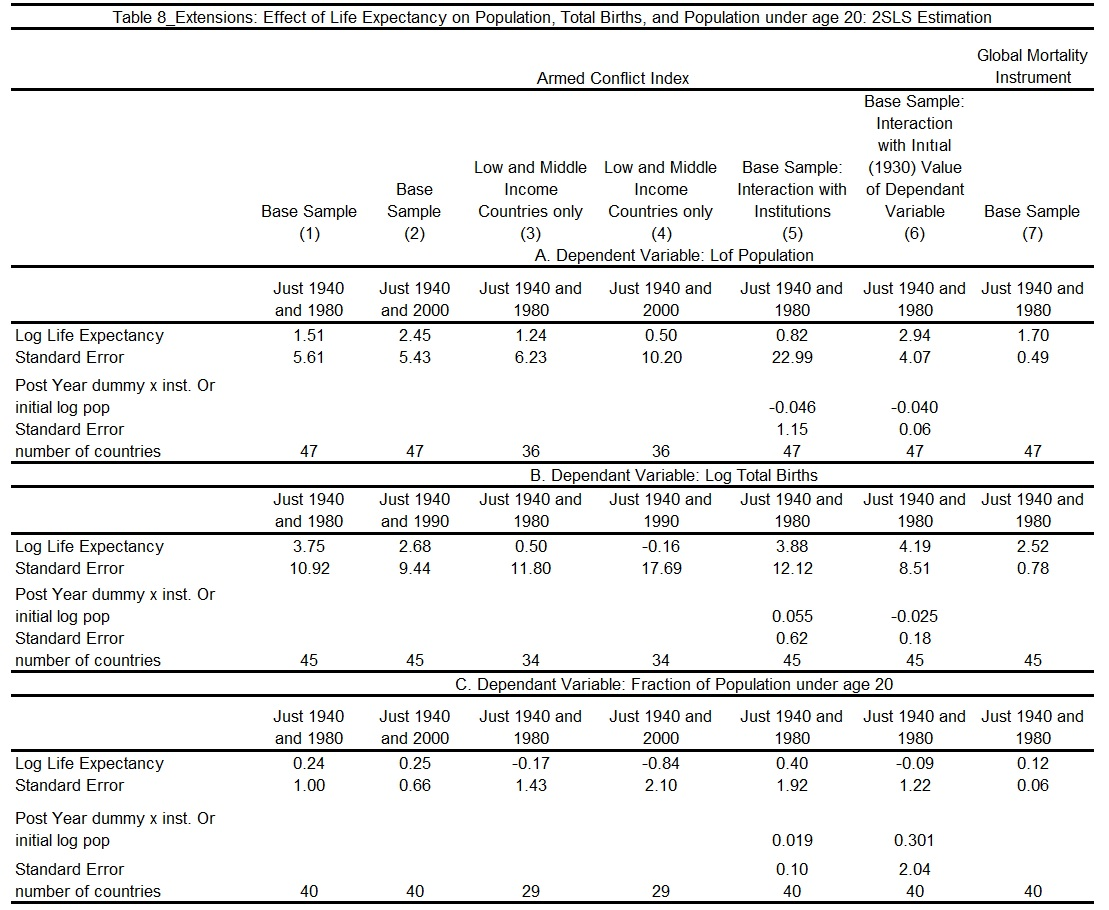
\includegraphics[width=\textwidth]{table8ex}
\label{table8ex}
\end{figure}
The main result of Table 8-Extensions are in line with Acemoglu and Johnson: there is a positive relationship between life expectancy and population growth. In fact, using armed conflict index magnifies the positive impact of life expectancy on population. 

When we compare Table 9 and Table 9-Extensions, excluding the base sample in column $(1)$, there is a positive relationship between log GDP and life expectancy. Hence, we are still following Acemoglu and Johnson. However, when we look at the log GDP per capita and log GDP per working age population, we could obtain some positive results if the country is not a rich country (Look at column $(3)$ and $(4)$). The other parts are more or less similar in term of the relationship between life expectancy and GDP.
\begin{figure} [H]
\centering
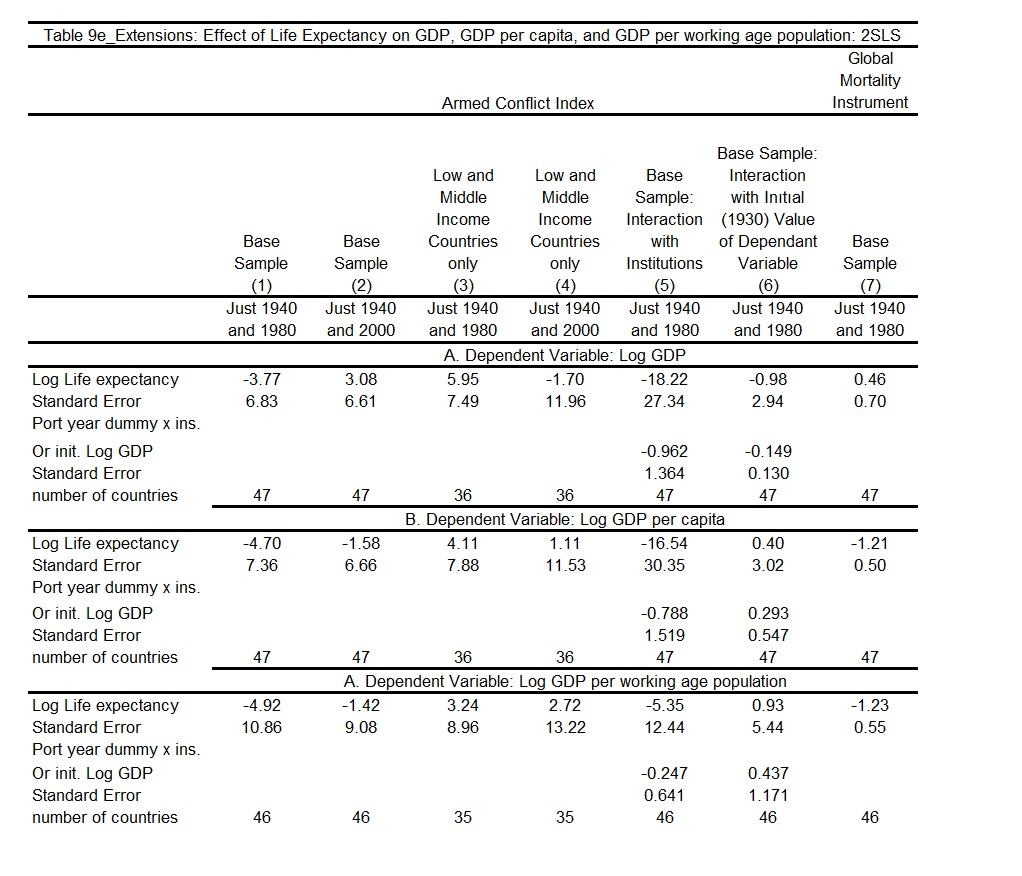
\includegraphics[width=\textwidth]{table9ex}
\label{table9ex}
\end{figure}
To sum up, based on the results we obtain in table 8-Extensions and Table 9-Extensions, we can conclude that low and middle income countries experience economic growth as the life expectancy of individuals increase. This conclusion is sensible in the following sense: We know that developed countries are by definition are more close to steady state and any exogenous change in the economy make the economy converge to steady state slowly. On the the other hand, speed of convergence of low and middle income countries are faster. So, any exogenous change in the economy will have a magnified effect. From this perspective, it may be the case that productivity effect has a magnified impact on economic growth as a result of better health conditions and dominate the population effect. 

Although we get a desirable result for low and middle income countries, the question is still valid for rich countries. It is apparent that introducing a new instrument did not produce a positive relationship between life expectancy and economic growth for rich countries so further study may include examining different perspectives to fully understand the relationship in rich countries.

\section*{Reference}
Acemoglu, D. and Johnson, S., (December 2007) \emph{Disease and Development: The effect of Life Expectancy on Economic Growth}, Journal of Political Economy 115, pp.928-985
\end{document}